\documentclass[../main.tex]{subfiles}
\graphicspath{{\subfix{../Figures/}}}
\begin{document}
    \begin{frame}{Discussion about leaking}         
        Leaking is indeed still an open problem in hypergraphs. In particular, it is indeed possible to prove that 
        \begin{block}{Leaking starting from the stationary distribution on a set $S$}
			$\chi_S^T(\prod_{t'\leq t}(D_S M_{t'})) \psi_S \geq 1 - t\phi(S)$
        \end{block}
    	
    	\begin{columns}
    		\column{0.5\textwidth}		
	    		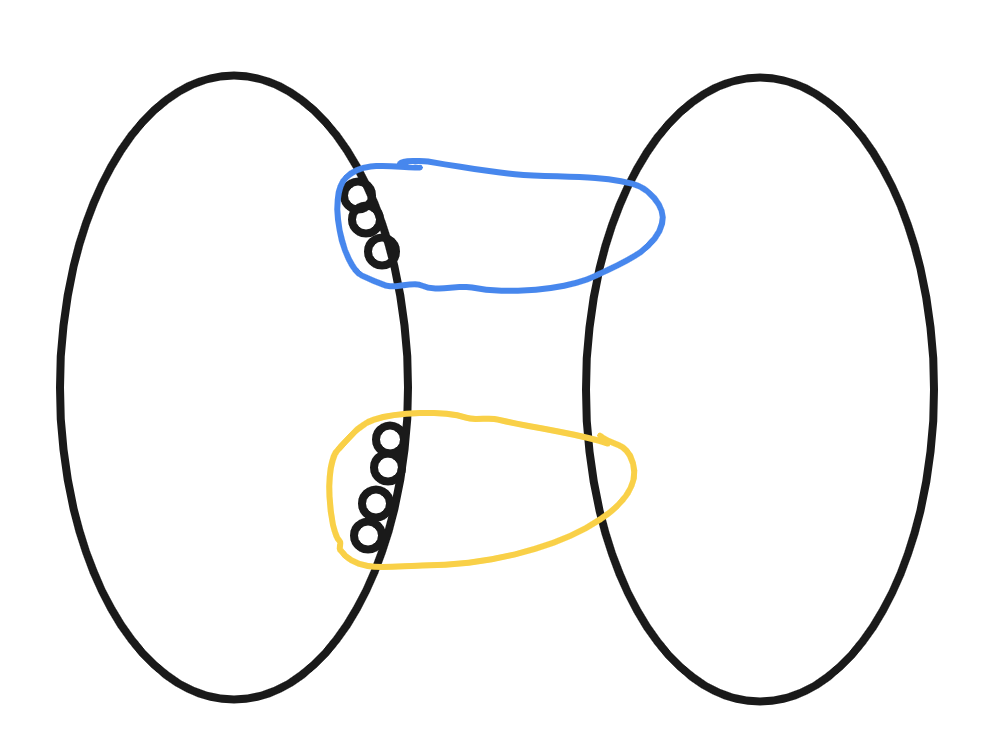
\includegraphics[width=0.8\textwidth]{leaking_hypergraph}
    		\column{0.5\textwidth}
    			When starting with probability centered in single vertices, instead, we count crossing hyperedges up to $r$ times (only for the first iteration though).
		\end{columns}
    \end{frame}

	\begin{frame}{Future work}
		For $r$-uniform hypergraphs we could prove an improved mixing theorem by a factor $r$, and a worse leaking theorem by a factor $r$. This would give a proper local clustering algorithm with the same guarantees as in graphs.
	\end{frame}
	
\end{document}